\chapter{Liouville's Theorem and Hamiltonian Flow}

\lectureoverview{Hamilton's equations do more than repackage the equations of
motion.  They define a velocity field on phase space whose divergence vanishes.
That simple cancellation is Liouville's theorem: Hamiltonian evolution
preserves phase-space volume.  We shall reach it in the order in which its
meaning becomes visible---first energy conservation, then constant-energy
surfaces, then a fluid of possible initial conditions, and finally the contrast
between volume-preserving flow and a dissipative sink.  The same language leads
naturally to Poisson brackets.}

\section{Why Another Form of Mechanics?}

The theorem we want is the continuous classical counterpart of the reversible
state diagrams introduced at the beginning of the course.  In a reversible
discrete law, every state has one arrow entering and one arrow leaving.  The
present is enough to determine both the next state and the preceding one.  A
bad law sends many states into one sink: the future may be determined, but the
past is no longer recoverable.

Liouville's theorem says what becomes of that distinction when the set of
states is a continuous phase space.  The phrase replacing one arrow in and one
arrow out will be \emph{as much flow in as flow out}.  Before that phrase can be
made mathematical, however, we need to reconstruct the flow from Hamilton's
equations.

There is a historical puzzle in doing so.  Hamilton, Jacobi, Lagrange, and
Poisson built elaborate and beautiful forms of classical mechanics without
knowing the quantum theory in which those forms would become indispensable.
Newton had a direct target: planetary motion.  Lagrange and Hamilton also had
physical problems before them, but they pursued analogies and structures far
beyond any one orbit.  Stationary action in mechanics resembled least-time
principles in optics; ray motion and particle motion could be put into parallel
mathematical forms.  They simplified, rearranged, and unified the equations
because the structures themselves appeared to contain physics.

We now know that this instinct was extraordinarily productive.  Logically,
many features of classical mechanics can be understood as limits of quantum
mechanics.  Historically, the order was reversed: the classical structures
were found first, and only much later did their deeper use become clear.  A
provocative joke attributed to Feynman made the point by contrasting
mathematics pursued internally with physics constrained by an external partner,
the physical world.  The joke is not an argument, but the distinction is useful:
formal beauty matters here because nature repeatedly selects these formal
structures.

\begin{classroomqa}
  \audiencequestion{Did Newton have the modern concept of kinetic energy, and
  where did the concept of energy begin?
  \lecturetimestamp{00:04:24--00:05:50}}
  \lecturerresponse{Newton's mechanics was organized around force and motion,
  not around a mature general energy principle.  The exact historical priority
  is not settled in the discussion.  Leibniz's \emph{vis viva},
  \(\sum_i m_i v_i^2\), was an important predecessor and equals twice the
  modern kinetic energy.  Later work on heat made the conversion between heat
  and mechanical work central.  Early caloric theories treated heat as a
  conserved substance, so the modern idea of interchangeable forms of energy
  emerged only gradually.}
\end{classroomqa}

\section{Hamilton's Equations and Energy Conservation}

Let a system have \(n\) canonical pairs,
\begin{equation}
  (q_i,p_i),\qquad i=1,\ldots,n.
  \label{eq:l7-canonical-pairs}
\end{equation}
There is one momentum for each coordinate and one coordinate for each momentum.
The law of motion is packaged in one function,
\begin{equation}
  H=H(q_1,\ldots,q_n,p_1,\ldots,p_n,t),
  \label{eq:l7-hamiltonian}
\end{equation}
and Hamilton's equations are
\begin{equation}
  \boxed{
  \dot q_i=\frac{\partial H}{\partial p_i},
  \qquad
  \dot p_i=-\frac{\partial H}{\partial q_i}.}
  \label{eq:l7-hamilton-equations}
\end{equation}
The sign is part of the canonical structure.  The \(q\)-equation carries the
plus sign; the \(p\)-equation carries the minus sign.

\begin{figure}[htbp]
  \centering
  
\includegraphics[width=0.82\textwidth]{lecture_07_figure_02.png}
  \caption{Canonical variables, the function \(H(q,p)\), and the
  momentum-side Hamilton equation at the beginning of the recap.}
  \lectureframe{00:07:29}
\end{figure}

Although the equations come in indexed pairs, the dynamics need not separate
pair by pair.  The Hamiltonian may couple every \(q_i\) and \(p_i\), so
\(\dot p_1\), for example, may depend on the state of the entire system.

\begin{classroomqa}
  \audiencequestion{Is the presentation now axiomatic?  What relation between
  \(p\) and \(q\) has been assumed?
  \lecturetimestamp{00:17:08--00:18:18}}
  \lecturerresponse{Hamilton's equations define the formal theory once
  \(H(q,p)\) and the canonical pairs are specified.  There is no universal
  extra assumption \(p=m\dot q\).  That relation holds for an ordinary
  Cartesian particle with quadratic kinetic energy, but other coordinates and
  other Hamiltonians give other momentum--velocity relations.  The equations
  themselves supply the relation through
  \(\dot q_i=\partial H/\partial p_i\).  Whether a proposed Hamiltonian is
  realized in nature is a further physical question.}
\end{classroomqa}

We can now recover energy conservation in one line of reasoning.  Along a
trajectory, the total derivative of \(H\) is
\begin{equation}
  \frac{dH}{dt}
  =
  \sum_i\left(
    \frac{\partial H}{\partial q_i}\dot q_i
    +\frac{\partial H}{\partial p_i}\dot p_i
  \right)
  +\frac{\partial H}{\partial t}.
  \label{eq:l7-total-h-derivative}
\end{equation}
The last term means explicit time dependence at fixed \(q\) and \(p\), perhaps
because an externally prescribed parameter is changing.  Substituting
Eq.~\eqref{eq:l7-hamilton-equations},
\begin{align}
  \frac{dH}{dt}
  &=
  \sum_i\left[
    \frac{\partial H}{\partial q_i}
    \frac{\partial H}{\partial p_i}
    -\frac{\partial H}{\partial p_i}
    \frac{\partial H}{\partial q_i}
  \right]
  +\frac{\partial H}{\partial t}\\
  &=\frac{\partial H}{\partial t}.
  \label{eq:l7-h-energy-rate}
\end{align}
Every term in the sum cancels its partner.  Consequently,
\begin{equation}
  \frac{\partial H}{\partial t}=0
  \quad\Longrightarrow\quad
  \frac{dH}{dt}=0.
  \label{eq:l7-energy-conservation}
\end{equation}
For a closed, time-translation-invariant system, the Hamiltonian is conserved
and is the energy.

\begin{classroomqa}
  \audiencequestion{What changes if the Hamiltonian depends explicitly on
  time? \lecturetimestamp{00:10:32--00:12:33}}
  \lecturerresponse{Then Eq.~\eqref{eq:l7-h-energy-rate} still holds, but the
  subsystem energy need not be constant.  An explicit time dependence usually
  represents an omitted driver exchanging energy with the system.  If that
  driver is promoted to a dynamical part of a larger closed system, the larger
  Hamiltonian can again be time independent and its total energy conserved.}
\end{classroomqa}

\section{Energy as Geometry in Phase Space}

Suppose now that \(H\) has no explicit time dependence.  The initial condition
fixes a number \(E\), and the phase point remains on
\begin{equation}
  H(q,p)=E.
  \label{eq:l7-energy-surface}
\end{equation}
Phase space has \(2n\) dimensions.  At regular points, one equation among its
coordinates defines a \((2n-1)\)-dimensional hypersurface.  Different values
of \(E\) give different hypersurfaces.  They need not be closed or compact;
energy conservation says only that a trajectory beginning on one of them
never leaves it.

For the adapted harmonic oscillator from the preceding lecture,
\begin{equation}
  H=\frac{\omega}{2}(p^2+q^2).
  \label{eq:l7-oscillator-hamiltonian}
\end{equation}
Thus each constant-energy set is a circle,
\begin{equation}
  p^2+q^2=\frac{2E}{\omega}.
  \label{eq:l7-oscillator-circle}
\end{equation}

\begin{figure}[htbp]
  \centering
  
\includegraphics[width=0.84\textwidth]{lecture_07_figure_04.png}
  \caption{The \(2n\)-dimensional phase-space sketch and the harmonic
  oscillator Hamiltonian used to introduce constant-energy surfaces.}
  \lectureframe{00:15:20}
\end{figure}

The equations of motion,
\begin{equation}
  \dot q=\omega p,\qquad \dot p=-\omega q,
  \label{eq:l7-oscillator-flow}
\end{equation}
make the point move clockwise around its circle.  The energy equation tells us
which curve contains the motion; Hamilton's equations tell us the direction
and speed along that curve.

\begin{figure}[htbp]
  \centering
  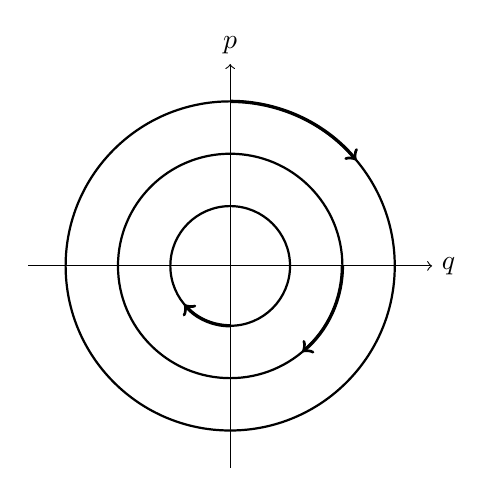
\begin{tikzpicture}[scale=0.95]
    \draw[->] (-2.7,0) -- (2.7,0) node[right] {\(q\)};
    \draw[->] (0,-2.7) -- (0,2.7) node[above] {\(p\)};
    \draw[thick] (0,0) circle (0.8);
    \draw[thick] (0,0) circle (1.5);
    \draw[thick] (0,0) circle (2.2);
    \draw[->,very thick] (0,2.2) arc[start angle=90,end angle=40,radius=2.2];
    \draw[->,very thick] (1.5,0) arc[start angle=0,end angle=-50,radius=1.5];
    \draw[->,very thick] (0,-0.8) arc[start angle=-90,end angle=-140,radius=0.8];
  \end{tikzpicture}
  \caption{Constant energy gives the circles; the oscillator equations give
  the clockwise tangent flow.}
\end{figure}

\begin{classroomqa}
  \audiencequestion{Are Hamilton's two equations and \(H=E\) several versions
  of the same equation?
  \lecturetimestamp{00:15:53--00:17:06}}
  \lecturerresponse{No.  Hamilton's equations are the two first-order laws of
  motion for one canonical pair.  They imply \(dH/dt=0\), from which
  \(H=E\) follows.  The value of \(E\) is selected by the initial condition.
  The equation \(H=E\) identifies a surface; it does not by itself specify the
  velocity along that surface.}
\end{classroomqa}

\section{From One State to a Flow of States}

Instead of following one initial condition, sprinkle phase space with every
possible initial condition and start the clock.  Each point is a complete
possible state, and each state moves according to Hamilton's equations.  The
sprinkling can be imagined as a dust or an imaginary fluid.  Nothing material
is being poured into phase space; the fluid is a way to see all trajectories
at once.

The phase-space velocity field is
\begin{equation}
  \mathbf V(q,p,t)
  =
  (\dot q_1,\ldots,\dot q_n,\dot p_1,\ldots,\dot p_n).
  \label{eq:l7-phase-velocity}
\end{equation}
For one canonical pair we write
\begin{equation}
  V_q=\dot q=\frac{\partial H}{\partial p},
  \qquad
  V_p=\dot p=-\frac{\partial H}{\partial q}.
  \label{eq:l7-phase-components}
\end{equation}
At each point the Hamiltonian assigns a vector telling the phase point where
to go next.  If \(H\) is time independent, the vector field is stationary:
returning to the same phase point gives the same velocity.  If \(H\) depends
on time, the vector field itself changes with time, but it is still defined at
each instant.

\begin{figure}[htbp]
  \centering
  
\includegraphics[width=0.84\textwidth]{lecture_07_figure_05.png}
  \caption{The harmonic-oscillator velocity field.  The vectors are tangent
  to the circles and become shorter toward the origin.}
  \lectureframe{00:24:50}
\end{figure}

For the harmonic oscillator every radius turns with angular speed \(\omega\).
Points near the origin have smaller linear speed because they travel a shorter
circle in the same period.  The entire dust therefore rotates as a rigid
carousel.

\begin{classroomqa}
  \audiencequestion{Does rigid rotation mean that all oscillator trajectories
  have the same period? \lecturetimestamp{00:21:10--00:21:42}}
  \lecturerresponse{Yes.  That amplitude independence is the defining special
  property of the harmonic oscillator.  Every circle is traversed with the
  same angular frequency \(\omega\), even though the magnitude of the
  phase-space velocity is smaller on a smaller circle.}
\end{classroomqa}

\begin{classroomqa}
  \audiencequestion{Is the phase-space velocity the same at every point?
  \lecturetimestamp{00:24:29--00:25:37}}
  \lecturerresponse{No.  Both its direction and magnitude generally vary with
  position.  For the oscillator the vector is tangent to the local circle and
  has magnitude \(\omega\sqrt{p^2+q^2}\).  A vector field means one assigned
  vector at every point, not one identical vector copied everywhere.}
\end{classroomqa}

\begin{classroomqa}
  \audiencequestion{What exactly are the particles and density of this
  imaginary fluid? \lecturetimestamp{00:56:03--00:58:40}}
  \lecturerresponse{Each point is one complete state of the whole mechanical
  system.  It is not one physical particle.  Five particles moving in one
  spatial dimension require five positions and five momenta, hence a
  ten-dimensional phase space; in three dimensions they require thirty
  dimensions.  The dust is an ensemble of alternative states.  If the fluid
  picture is distracting, simply take a region of initial conditions, evolve
  every point in it, and compare its phase-space volume before and after.}
\end{classroomqa}

\section{Compression and Divergence}

To ask whether this imaginary fluid loses volume, begin in one dimension.
Let points on a line move with velocity \(v(x)\).  Two nearby points separated
by \(\delta x\) have a velocity difference
\begin{equation}
  \delta v \simeq \frac{dv}{dx}\,\delta x.
  \label{eq:l7-one-dimensional-strain}
\end{equation}
If \(dv/dx>0\), the point ahead moves faster and the interval stretches.  If
\(dv/dx<0\), it compresses.  A stationary one-dimensional incompressible flow
therefore obeys
\begin{equation}
  \frac{dv}{dx}=0.
  \label{eq:l7-one-dimensional-incompressible}
\end{equation}

\begin{figure}[htbp]
  \centering
  
\includegraphics[width=0.84\textwidth]{lecture_07_figure_06.png}
  \caption{The one-dimensional construction leading to \(dv/dx\) as the
  local stretching or compression rate.}
  \lectureframe{00:30:20}
\end{figure}

There are two equivalent viewpoints.  We may follow a material interval and
ask whether its length changes.  Or we may hold a small interval fixed and
ask whether the amount entering per unit time equals the amount leaving.
The first follows the fluid; the second watches it pass.

In more than one dimension a region may stretch along one axis and compress
along another without changing total volume.  For a velocity field
\(\mathbf V=(V_x,V_y,V_z)\), the relevant local rate is the divergence,
\begin{equation}
  \nabla\cdot\mathbf V
  =
  \frac{\partial V_x}{\partial x}
  +\frac{\partial V_y}{\partial y}
  +\frac{\partial V_z}{\partial z}.
  \label{eq:l7-spatial-divergence}
\end{equation}
Positive divergence is local expansion, negative divergence is local
contraction, and incompressibility is
\begin{equation}
  \nabla\cdot\mathbf V=0.
  \label{eq:l7-zero-divergence}
\end{equation}
Equal inflow and outflow through a fixed small box is the same local statement
as preservation of the volume of a moving small box.

\begin{figure}[htbp]
  \centering
  
\includegraphics[width=0.86\textwidth]{lecture_07_figure_07.png}
  \caption{A two-dimensional box, its flow components, and the sum of
  same-coordinate derivatives that defines divergence.}
  \lectureframe{00:35:30}
\end{figure}

\begin{classroomqa}
  \audiencequestion{Are we discussing a fluid in ordinary space or a flow in
  phase space? \lecturetimestamp{00:34:27--00:34:40}}
  \lecturerresponse{The divergence argument is first a general fluid argument.
  We shall apply it to the even-dimensional phase space, where the coordinate
  directions are the \(q_i\) and \(p_i\), and the velocity components are
  \(\dot q_i\) and \(\dot p_i\).}
\end{classroomqa}

Now return to the discrete state maps.  In a reversible cycle, every node has
one arrow in and one arrow out, and a chosen collection of states retains the
same number of members as it evolves.  In a sink, many arrows enter and too
few leave; several alternatives become indistinguishable.

\begin{figure}[htbp]
  \centering
  
\includegraphics[width=0.80\textwidth]{lecture_07_figure_08.png}
  \caption{The discrete sink used to reconnect divergence with the
  first-lecture test for reversible laws.}
  \lectureframe{00:40:15}
\end{figure}

The continuous question is now exact: does Hamiltonian flow have zero
divergence, so that a small region of distinguishable states never gets
squashed into a smaller phase-space volume?

\section{Liouville's Theorem}

\begin{theorem}[Liouville's theorem]
For a smooth Hamiltonian system, the canonical phase-space velocity field has
zero divergence:
\begin{equation}
  \sum_i\left(
    \frac{\partial\dot q_i}{\partial q_i}
    +\frac{\partial\dot p_i}{\partial p_i}
  \right)=0.
  \label{eq:l7-liouville-divergence}
\end{equation}
Equivalently, Hamiltonian evolution preserves the canonical phase-space volume
\(dq_1\cdots dq_n\,dp_1\cdots dp_n\).
\end{theorem}

\begin{classroomqa}
  \audiencequestion{Are the components called \(V\) simply the \(p\)-dots and
  \(q\)-dots? \lecturetimestamp{00:42:20--00:43:22}}
  \lecturerresponse{Yes.  For one pair,
  \(V_q=\dot q\) and \(V_p=\dot p\).  Lining up all such derivatives gives the
  velocity vector of the flow in the full phase space.}
\end{classroomqa}

For one canonical pair, Hamilton's equations give
\begin{equation}
  V_p=-\frac{\partial H}{\partial q},
  \qquad
  V_q=\frac{\partial H}{\partial p}.
  \label{eq:l7-liouville-components}
\end{equation}
The divergence is therefore
\begin{align}
  \frac{\partial V_p}{\partial p}
  +\frac{\partial V_q}{\partial q}
  &=
  -\frac{\partial}{\partial p}
    \left(\frac{\partial H}{\partial q}\right)
  +\frac{\partial}{\partial q}
    \left(\frac{\partial H}{\partial p}\right)\\
  &=
  -\frac{\partial^2H}{\partial p\,\partial q}
  +\frac{\partial^2H}{\partial q\,\partial p}
  =0.
  \label{eq:l7-liouville-proof}
\end{align}

\begin{figure}[htbp]
  \centering
  
\includegraphics[width=0.86\textwidth]{lecture_07_figure_09.png}
  \caption{The finite-difference rectangle used to explain why smooth mixed
  partial derivatives commute.}
  \lectureframe{00:47:30}
\end{figure}

The equality of mixed partial derivatives can be seen with four nearby points
\(A,B,C,D\) at the corners of a small rectangle in the \(q\)-\(p\) plane.
Taking a \(q\)-difference and then a \(p\)-difference produces, apart from the
two small side lengths,
\begin{equation}
  F(B)+F(D)-F(A)-F(C).
  \label{eq:l7-finite-difference-combination}
\end{equation}
Taking the differences in the opposite order produces the same combination.
In the small-rectangle limit this is
\(\partial_p\partial_qF=\partial_q\partial_pF\), provided the required
derivatives are continuous.

\begin{figure}[htbp]
  \centering
  
\includegraphics[width=0.88\textwidth]{lecture_07_figure_10.png}
  \caption{The canonical divergence after Hamilton's equations have reduced
  it to two mixed derivatives with opposite signs.}
  \lectureframe{00:50:20}
\end{figure}

For many degrees of freedom, the same cancellation occurs for every canonical
pair:
\begin{align}
  \sum_i\left(
    \frac{\partial\dot p_i}{\partial p_i}
    +\frac{\partial\dot q_i}{\partial q_i}
  \right)
  &=
  \sum_i\left(
    -\frac{\partial^2H}{\partial p_i\,\partial q_i}
    +\frac{\partial^2H}{\partial q_i\,\partial p_i}
  \right)\\
  &=0.
  \label{eq:l7-many-pair-proof}
\end{align}
Stretching in one canonical direction is balanced by compression in its
conjugate direction.  This pairwise cancellation is stronger structure than a
coincidental cancellation among unrelated axes.

\begin{classroomqa}
  \audiencequestion{Is the summation over all canonical pairs understood?
  \lecturetimestamp{00:52:00--00:52:36}}
  \lecturerresponse{Yes.  Equation~\eqref{eq:l7-many-pair-proof} is summed over
  \(i\), and the two mixed derivatives cancel separately within each
  \(q_i,p_i\) pair.}
\end{classroomqa}

\begin{classroomqa}
  \audiencequestion{The displayed divergence looks Cartesian.  Does the
  theorem survive a change of coordinates?
  \lecturetimestamp{00:52:50--00:53:22,\allowbreak\ 00:58:18--00:58:40}}
  \lecturerresponse{The natural statement is made in canonical coordinates
  and with the canonical volume element
  \(dq_1\cdots dq_n\,dp_1\cdots dp_n\).  A canonical, or symplectic,
  transformation changes coordinates and momenta together and preserves that
  volume.  In arbitrary noncanonical coordinates, a Jacobian factor belongs
  in the volume measure; the naive product of coordinate increments need not
  be invariant.}
\end{classroomqa}

\begin{classroomqa}
  \audiencequestion{Does Liouville's theorem require a time-independent
  Hamiltonian? \lecturetimestamp{00:53:43--00:55:51}}
  \lecturerresponse{No.  Energy conservation required
  \(\partial H/\partial t=0\), but the divergence proof differentiates only
  with respect to \(q_i\) and \(p_i\) at a fixed time.  The mixed partials still
  cancel for \(H(q,p,t)\).  A time-dependent Hamiltonian therefore generates a
  time-dependent but instantaneously volume-preserving canonical flow.}
\end{classroomqa}

\section{What Volume Preservation Does and Does Not Mean}

Take any small region \(R_0\) of initial conditions and evolve every point for
a time \(t\).  Liouville's theorem says
\begin{equation}
  \operatorname{Vol}(R_t)=\operatorname{Vol}(R_0).
  \label{eq:l7-volume-preservation}
\end{equation}
The region may move, rotate, shear, and stretch into a long filament.  Its
volume, not its shape, is protected.  Distinct phase points cannot coalesce in
a finite smooth Hamiltonian evolution.

For finite times, a smooth Hamiltonian flow is an invertible map with a smooth
inverse obtained by evolving backward.  This also explains the classroom
claim that a connected blob cannot pinch into disconnected pieces: the flow
deforms the region continuously and preserves its topology, even though an
extremely thin neck may make two lobes look separated at finite resolution.

\begin{figure}[htbp]
  \centering
  
\includegraphics[width=0.86\textwidth]{lecture_07_figure_12.png}
  \caption{Possible deformations of one phase-space region.  A smooth
  Hamiltonian flow may produce a thin neck, but not a genuine finite-time
  break into independently evolved pieces.}
  \lectureframe{01:04:55}
\end{figure}

\begin{classroomqa}
  \audiencequestion{Can a phase-space region pinch off and split into two
  pieces? \lecturetimestamp{01:04:10--01:05:49}}
  \lecturerresponse{Not under a smooth deterministic Hamiltonian flow for a
  finite time.  At a hypothetical pinch point there is still one phase-space
  point and one assigned velocity, not two incompatible directions.  The
  region can develop a very long, narrow connecting filament, but the
  evolution remains one-to-one and does not tear it.}
\end{classroomqa}

\begin{classroomqa}
  \audiencequestion{Are two widely separated lobes of a stretched blob
  physically connected or quantum-entangled?
  \lecturetimestamp{01:08:01--01:09:16}}
  \lecturerresponse{No such physical connection is implied.  The blob is a set
  of alternative initial conditions, not one material object.  Calling it one
  region records the common set from which those states evolved; it says
  nothing about forces or quantum entanglement between them.}
\end{classroomqa}

\begin{classroomqa}
  \audiencequestion{What happens near the upright unstable equilibrium of a
  rigid pendulum?  Do clockwise and counterclockwise trajectories overlap?
  \lecturetimestamp{01:07:07--01:07:47}}
  \lecturerresponse{Nearby initial conditions can separate onto very different
  trajectories, producing the thin filaments just described.  They do not
  become the same phase point: the sign of the infinitesimal displacement or
  momentum distinguishes the two sides.  The exactly balanced state has its
  own uniquely determined motion, namely remaining at equilibrium in the ideal
  model.}
\end{classroomqa}

\subsection{Expansion in Position Space and Contraction in Momentum Space}

If a canonical transformation expands a range of positions by a factor \(a\),
the conjugate momentum scale contracts by the reciprocal factor:
\begin{equation}
  q\longrightarrow aq,
  \qquad
  p\longrightarrow \frac{p}{a},
  \qquad
  dq\,dp\longrightarrow dq\,dp.
  \label{eq:l7-canonical-scaling}
\end{equation}
This is the clean phase-space content behind the gas-expansion example.  In an
adiabatic expansion, the accessible ordinary-space region grows while typical
momenta fall and the gas cools.  A detailed thermodynamic relation depends on
dimension, the expansion protocol, and interactions; Liouville's theorem
supplies the volume constraint, not every thermodynamic coefficient.

\begin{classroomqa}
  \audiencequestion{Does the same reasoning apply to an expanding universe,
  even for a sudden expansion? \lecturetimestamp{00:53:23--00:56:00}}
  \lecturerresponse{Liouville's theorem applies whenever the complete dynamics
  is Hamiltonian, including explicitly time-dependent canonical variables.
  Expansion in position directions must be accompanied by the corresponding
  contraction in canonical-momentum directions.  A cosmological scale factor,
  a controlled expansion of a gas, and a freely exploding cloud are not the
  same physical process, however.  A Hubble-like correlation between distance
  and recession speed can arise because faster objects travel farther, whereas
  adiabatic cooling concerns contraction of the local momentum distribution.
  The theorem constrains the full phase-space map in either case.}
\end{classroomqa}

\begin{classroomqa}
  \audiencequestion{What practical use does Liouville's theorem have?
  \lecturetimestamp{01:06:16--01:07:04}}
  \lecturerresponse{It is central to statistical mechanics.  It controls how
  ensembles of microscopic states evolve and underlies the relation between
  phase-space volume and entropy.  The expansion and cooling of a gas is one
  immediate illustration; later it becomes a basic tool for equilibrium and
  nonequilibrium reasoning.}
\end{classroomqa}

\section{A Flow That Changes Shape Violently}

The harmonic oscillator preserves both area and shape because its flow is a
rigid rotation.  That is exceptional.  To separate volume preservation from
rigidity, take
\begin{equation}
  H=\lambda pq,
  \label{eq:l7-pq-hamiltonian}
\end{equation}
where \(\lambda\) has units of inverse time.  The lecture sets
\(\lambda=1\); retaining it makes the dimensions explicit.

\begin{figure}[htbp]
  \centering
  
\includegraphics[width=0.82\textwidth]{lecture_07_figure_03.png}
  \caption{The beginning of the \(H=pq\) example and the first phase-space
  velocity component.}
  \lectureframe{01:00:11}
\end{figure}

Hamilton's equations are
\begin{equation}
  \dot p=-\lambda p,
  \qquad
  \dot q=\lambda q,
  \label{eq:l7-pq-flow}
\end{equation}
with solutions
\begin{equation}
  p(t)=p_0e^{-\lambda t},
  \qquad
  q(t)=q_0e^{\lambda t}.
  \label{eq:l7-pq-solutions}
\end{equation}
A square patch is exponentially squeezed in \(p\) and stretched by the same
factor in \(q\):
\begin{equation}
  \Delta p(t)\Delta q(t)
  =
  \Delta p(0)\Delta q(0).
  \label{eq:l7-pq-area}
\end{equation}
Its divergence verifies the result locally,
\begin{equation}
  \frac{\partial\dot p}{\partial p}
  +\frac{\partial\dot q}{\partial q}
  =-\lambda+\lambda=0.
  \label{eq:l7-pq-divergence}
\end{equation}

\begin{figure}[htbp]
  \centering
  
\includegraphics[width=0.86\textwidth]{lecture_07_figure_11.png}
  \caption{A compact patch stretched into a long thin strip while preserving
  area under the \(H=pq\) flow.}
  \lectureframe{01:02:10}
\end{figure}

\begin{classroomqa}
  \audiencequestion{Since \(pq\) has units of action, is Liouville's theorem
  conservation of action? \lecturetimestamp{01:03:00--01:04:09}}
  \lecturerresponse{No.  The theorem conserves phase-space volume.  In one
  canonical pair, \(dq\,dp\) has units of action, and that dimensional fact
  foreshadows quantum mechanics, where phase-space cells are measured in units
  set by \(\hbar\).  But the product \(pq\) is not itself Hamilton's action
  functional, nor is it automatically angular momentum merely because the
  dimensions agree.}
\end{classroomqa}

The example also shows that angles need not be preserved.  A right-angle cross
with unequal components under the scaling in
Eq.~\eqref{eq:l7-pq-solutions} is sheared in its metric appearance, while area
remains unchanged.  Liouville's theorem is an area or volume theorem, not an
ordinary Euclidean rigidity theorem.

\section{Damping Produces a Sink}

To see what the theorem excludes, consider the reduced equation for a damped
oscillator,
\begin{equation}
  m\ddot x=-kx-c\dot x,
  \qquad c>0.
  \label{eq:l7-damped-newton}
\end{equation}
Let \(p=m\dot x\).  Then
\begin{equation}
  \dot x=\frac{p}{m},
  \qquad
  \dot p=-kx-\frac{c}{m}p.
  \label{eq:l7-damped-first-order}
\end{equation}
Without damping, the phase point circles the origin.  With damping, energy is
transferred into the microscopic degrees of freedom of the surrounding medium,
and the orbit spirals inward.

\begin{figure}[htbp]
  \centering
  
\includegraphics[width=0.84\textwidth]{lecture_07_figure_13.png}
  \caption{The damped oscillator equation and its inward spiral in the
  \(x\)-\(p\) plane.}
  \lectureframe{01:13:30}
\end{figure}

The divergence of this reduced two-dimensional flow is
\begin{equation}
  \frac{\partial\dot x}{\partial x}
  +\frac{\partial\dot p}{\partial p}
  =
  0-\frac{c}{m}<0.
  \label{eq:l7-damped-divergence}
\end{equation}
Every finite patch contracts.  The origin is a sink, the continuous analogue
of the many-arrows-in state map.

\begin{figure}[htbp]
  \centering
  
\includegraphics[width=0.88\textwidth]{lecture_07_figure_14.png}
  \caption{The damped phase-space velocity components used to obtain the
  negative divergence \(-c/m\).}
  \lectureframe{01:16:05}
\end{figure}

This does not mean that microscopic mechanics violates Liouville's theorem.
The two variables \(x,p\) omit the enormous number of environmental degrees of
freedom that receive the oscillator's energy.  The enlarged oscillator-plus-
environment system can be Hamiltonian and volume preserving even though its
reduced \(x,p\) description contracts.

\begin{classroomqa}
  \audiencequestion{Is the damped oscillator still described by Newton's
  equation, even though it is not Hamiltonian in this reduced phase space?
  \lecturetimestamp{01:20:09--01:21:12}}
  \lecturerresponse{Yes.  Newton's \(F=ma\) can include an empirically supplied
  drag force.  The elementary \(L=T-V\) and Hamiltonian description applies
  directly to conservative forces, and more general Lagrangians also handle
  some velocity-dependent forces.  A Markovian friction term for an isolated
  pair \(x,p\), however, is reduced dissipative dynamics, not a closed
  canonical Hamiltonian system.}
\end{classroomqa}

\begin{classroomqa}
  \audiencequestion{If the damped equations can be integrated backward with
  infinite precision, is information really lost?
  \lecturetimestamp{01:25:16--01:27:17}}
  \lecturerresponse{For any finite time the ideal differential equation still
  has an inverse, so exact data can be run backward.  The precise statement is
  that finite phase-space cells contract exponentially.  Recovering their past
  then requires exponentially increasing precision, and at infinite time all
  trajectories approach the sink.  This is the closest continuous classical
  analogue of the discrete loss-of-alternatives picture, not an assertion that
  two exact finite-time solutions literally become one.}
\end{classroomqa}

\begin{classroomqa}
  \audiencequestion{Can a vector field have zero divergence without coming
  from a Hamiltonian? \lecturetimestamp{01:18:21--01:22:34}}
  \lecturerresponse{Certainly.  Hamiltonian form is sufficient for zero
  divergence, not necessary.  An arbitrary incompressible velocity field can
  have zero divergence without being a canonical Hamiltonian field on that
  same space.  A three-dimensional incompressible fluid velocity field is the
  classroom example: three coordinates cannot themselves form canonical
  pairs.  Full fluid mechanics may possess more sophisticated
  infinite-dimensional Hamiltonian formulations, but that does not reverse
  the one-way implication being made here.}
\end{classroomqa}

\section{Further Distinctions Exposed by Questions}

\begin{classroomqa}
  \audiencequestion{How is motion on a constant-energy surface related to
  preservation of a whole phase-space volume?
  \lecturetimestamp{01:28:47--01:30:41}}
  \lecturerresponse{They are independent consequences of the Hamiltonian
  structure.  If \(H\) is time independent, each trajectory remains on its own
  energy surface.  A finite patch may cross many such surfaces; Liouville's
  theorem says that the volume of that entire patch is preserved.  For the
  harmonic oscillator the patch also keeps its shape because the flow is a
  rigid rotation.  The \(H=pq\) patch keeps only its area, not its shape.}
\end{classroomqa}

\begin{classroomqa}
  \audiencequestion{Where does mechanical work fit into the Hamiltonian
  account? \lecturetimestamp{01:30:44--01:32:57}}
  \lecturerresponse{Work describes energy transferred across a chosen system
  boundary.  An external agent can raise a weight or change a parameter and
  thereby change the subsystem energy; the energy it supplies is lost by the
  agent.  If both sides are included in one closed model, the emphasis returns
  to total energy conservation and exchange between subsystems.}
\end{classroomqa}

\begin{classroomqa}
  \audiencequestion{Does volume preservation also preserve topology and
  angles? \lecturetimestamp{01:33:00--01:33:37}}
  \lecturerresponse{A smooth finite-time Hamiltonian flow preserves topology
  because it is an invertible continuous deformation.  It does not generally
  preserve Euclidean angles or shape.  The oscillator's rigid rotation does,
  but the \(H=pq\) stretching demonstrates why that is a special case.}
\end{classroomqa}

\begin{classroomqa}
  \audiencequestion{Was the Legendre transformation omitted because it has no
  physical significance? \lecturetimestamp{01:33:43--01:34:48}}
  \lecturerresponse{No.  It is the useful transformation that exchanges the
  velocity description for the momentum description and produces
  \(H=\sum_i p_i\dot q_i-L\) when the map is regular.  The construction has
  already been used repeatedly even when its formal name was not emphasized;
  the detailed general theory is simply not needed for the present theorem.}
\end{classroomqa}

\section{Poisson Brackets: The Next Compression}

The final minutes return to the historical theme.  Nineteenth-century
mechanics repeatedly searched for compact structures linking apparently
different systems---mechanics and geometrical optics, particles and rays,
classical trajectories and wave-like descriptions.  Poisson brackets are
another such structure, and they become especially important in quantum
mechanics.

Let \(F(q,p)\) be any function on phase space.  It might be a coordinate, a
momentum, the product \(qp\), or angular momentum.  Along the motion,
\begin{equation}
  \frac{dF}{dt}
  =
  \sum_i\left(
    \frac{\partial F}{\partial q_i}\dot q_i
    +\frac{\partial F}{\partial p_i}\dot p_i
  \right).
  \label{eq:l7-f-time-derivative}
\end{equation}
Substitute Hamilton's equations:
\begin{equation}
  \frac{dF}{dt}
  =
  \sum_i\left(
    \frac{\partial F}{\partial q_i}
    \frac{\partial H}{\partial p_i}
    -
    \frac{\partial F}{\partial p_i}
    \frac{\partial H}{\partial q_i}
  \right).
  \label{eq:l7-f-hamiltonian-derivative}
\end{equation}

\begin{figure}[htbp]
  \centering
  
\includegraphics[width=0.88\textwidth]{lecture_07_figure_15.png}
  \caption{The chain rule for the time derivative of a general phase-space
  function \(F(q,p)\).}
  \lectureframe{01:42:40}
\end{figure}

The repeated antisymmetric combination deserves a name.  For any two
functions \(F\) and \(G\), define their Poisson bracket by
\begin{equation}
  \boxed{
  \{F,G\}
  =
  \sum_i\left(
    \frac{\partial F}{\partial q_i}
    \frac{\partial G}{\partial p_i}
    -
    \frac{\partial F}{\partial p_i}
    \frac{\partial G}{\partial q_i}
  \right).}
  \label{eq:l7-poisson-bracket}
\end{equation}

\begin{figure}[htbp]
  \centering
  
\includegraphics[width=0.86\textwidth]{lecture_07_figure_16.png}
  \caption{The two-function derivative combination as it is promoted to the
  Poisson bracket.}
  \lectureframe{01:44:15}
\end{figure}

Equation~\eqref{eq:l7-f-hamiltonian-derivative} becomes
\begin{equation}
  \boxed{\frac{dF}{dt}=\{F,H\}.}
  \label{eq:l7-hamiltonian-poisson-evolution}
\end{equation}
If \(F\) also depends explicitly on time, one adds
\(\partial F/\partial t\).  Taking \(F=q_i\) or \(F=p_i\) recovers Hamilton's
two equations, so Eq.~\eqref{eq:l7-hamiltonian-poisson-evolution} is a compact
form of the complete dynamics.

Notation can always be compressed artificially---one could square many
equations, add them, and call the result one equation.  That would hide rather
than reveal structure.  The Poisson bracket is useful for the opposite reason:
its algebra organizes time evolution, conserved quantities, and symmetry.
The next step is to develop that algebra and then use it for angular momentum,
whose structure will be central both in classical mechanics and in quantum
theory.

\section{The Continuous Meaning of Reversibility}

We can now state the chain of ideas without shortening it.  Hamilton's
equations conserve \(H\) when the Hamiltonian has no explicit time dependence,
so individual trajectories remain on constant-energy hypersurfaces.  The same
equations assign a velocity to every point of phase space.  The divergence of
that velocity vanishes because mixed partial derivatives cancel pairwise.
Consequently, a whole region of possible states preserves its canonical
volume.

That is the continuous version of one arrow in and one arrow out.  Shape can
change, angles can change, and neighboring trajectories can separate
enormously.  What cannot happen in a smooth closed Hamiltonian description is
the compression of a finite collection of alternatives into a smaller
phase-space volume.  The \(H=pq\) flow demonstrates the freedom to stretch;
the reduced damped oscillator demonstrates the sink that appears once the
Hamiltonian conditions are abandoned.  Poisson brackets then condense the same
dynamics into the statement that the Hamiltonian generates every time
derivative.
